\documentclass{article}
\usepackage{tcolorbox}
\usepackage{hyperref} %for better referencing
\title{\textbf{Manual for the freq\_map() function}}
\author{Chitran Ghosal}

%%PAGE GEOMETRY and PAGE SETUP, as in header/footer/footnote
%%-----------------------------------------------------------------------
%%-----------------------------------------------------------------------
\usepackage[a4paper, bindingoffset=6mm,
headheight=15.2pt % use geometry to change the head height
]{geometry}

\usepackage[headsepline,automark,autooneside=false]{scrlayer-scrpage}% sets pagestyle scrheadings automatically
%\renewcommand*\chaptermarkformat{}% remove chapter number from header entry
%\renewcommand*\sectionmarkformat{}% remove section number from header entry

\clearpairofpagestyles% before setting the new contents of header and footer
\cfoot*{\pagemark}
\ihead{\rightmark}
\ohead{\leftmark}
\addtokomafont{pageheadfoot}{\upshape}

% page style empty in TOC, LOF, LOT and all other lists under controll of  package tocbasic
%\AfterTOCHead{\thispagestyle{empty}\pagestyle{empty}}
%\AfterStartingTOC{\thispagestyle{empty}}

\usepackage{blindtext}% only for dummy text

\usepackage[bottom]{footmisc}                    %createsfootnotes
%%-----------------------------------------------------------------------
%%-----------------------------------------------------------------------

%%MATHEMATICAL PACKAGES
%%-----------------------------------------------------------------------
%%-----------------------------------------------------------------------
\usepackage{physics,amsthm, amsmath,esint}
\usepackage{amssymb}
\usepackage{amsfonts}
\usepackage{tcolorbox}
%%-----------------------------------------------------------------------
%%-----------------------------------------------------------------------

%%GRAPHICS PACKAGES
%%----------------------------------------------------------------------
%%----------------------------------------------------------------------
\usepackage{graphicx}               %needed for the insertion of graphics, remove draft for final script.
\graphicspath{{./images/}}            %needed for choosing the image path
\usepackage{caption}             %needed for captioning of a single image
\captionsetup{justification = raggedright, singlelinecheck = false} %forces left-alignment of captions
\usepackage{subcaption}         %needed for allowing 'sub'-captioning of multiple-images
%\setcapindent{2cm}                   %indents the caption borders to zero
\usepackage{float}	                         %allows using [H] for images
\usepackage[font={small}]{caption} %image captions in different fonts
%\usepackage{float}
%\floatstyle{boxed} 
%\restylefloat{figure}          %defines a border for all the float images
%%-----------------------------------------------------------------------
%%-----------------------------------------------------------------------



%%PACKAGE FOR APPENDICES
%%-----------------------------------------------------------------------
%%-----------------------------------------------------------------------
\usepackage[toc,page]{appendix}
%%-----------------------------------------------------------------------
%%-----------------------------------------------------------------------

%%PACKAGE FOR CODE INDENTATION
%%-----------------------------------------------------------------------
%%-----------------------------------------------------------------------
\usepackage{listings}
\usepackage{color}
%\usepackage[svgnames]{xcolor} %needed for RStudio code coloration
\lstset{language=R,
	basicstyle=\small\ttfamily,
	stringstyle=\color{DarkGreen},
	otherkeywords={0,1,2,3,4,5,6,7,8,9},
	morekeywords={TRUE,FALSE,T,F},
	deletekeywords={data,frame,length,as,character},
	keywordstyle=\color{blue},
	commentstyle=\color{DarkGreen},
}  %RStudio code lsiting
%\usepackage{color}

\definecolor{dkgreen}{rgb}{0,0.6,0}
\definecolor{gray}{rgb}{0.5,0.5,0.5}
\definecolor{mauve}{rgb}{0.58,0,0.82}

\lstset{frame=tb,
	language=Python,
	aboveskip=3mm,
	belowskip=3mm,
	showstringspaces=false,
	columns=flexible,
	basicstyle={\small\ttfamily},
	numbers=none,
	numberstyle=\tiny\color{gray},
	keywordstyle=\color{blue},
	commentstyle=\color{dkgreen},
	stringstyle=\color{mauve},
	breaklines=true,
	breakatwhitespace=true,
	tabsize=3
}
%%--------------------------------------------------------------------------
%%--------------------------------------------------------------------------

%%PACKAGE FOR SI UNITS
%%--------------------------------------------------------------------------
%%--------------------------------------------------------------------------
\usepackage{siunitx}
%%--------------------------------------------------------------------------
%%--------------------------------------------------------------------------
\begin{document}
	\maketitle
	\section{Abstract}
	This manual shows how to use the \textit{freq\_map()} package for mapping intensity dependence of a certain spectral window(in fourier space) in real space. This frequency mapping is similar to how dark-field microscopy is carried out in Low Energy Electron Microscopy(LEEM).  
	\section{Introduction}
	Often, within the parlance of data, the obtained data contains a range of periodicities. The obvious solution is to look at a frequency domain representation(Fourier Transform) of the signals in question. However, this makes sense when the frequency composition of the signal is uniform throughout the sample. In reality this is not the case.\\
	\\
	In the event of much more real signals, example audio signals or sunlight, the fourier space also isn't comprised of individual signal frequencies, rather they form a continuum in frequency space. In this case it makes sense to be interseted in the composition of the signal in real space(with respect to a given spectral-frequency window). The function \textit{freq\_map()} aims to solve this problem of frequency (window) mapping.
	\section{Examples}
	In the examples that follow, the use-cases and the proof of concept of the \textit{freq\_map()} package are shown
	\subsection{Example 1}
	The code in  listing.\ref{lst:cb1} is used to build a noisy mix of three sine waves with $\omega = 2\pi f$. With $f$ being chosen from 1000\si[]{Hz}, 5000\si[]{Hz} and 7734\si{Hz}.
	 \begin{lstlisting}[language=R, label={lst:cb1}, caption={code for simulating three frequency signal in fig.\ref{F1a} and its fourier transform in fig.\ref{F1b}}, captionpos=b]
	 	rm(list=ls())
	 	library('StatsChitran') #Call library
	 	ClearPlot() #Clear the plot
	 	t <- seq(0,10, by=1/60000) #define the time axis
	 	fcomp <- c(1000, 5000, 7734) #set which frequencies to build
	 	Y <- 3*sin(2*pi*fcomp[1]*t)*gauss(t, amp =5, sig = 0.7, mu=1 ) + 5*sin(2*pi*fcomp[2]*t)*gauss(t, amp = 4, sig = 1, mu=3) + 4*sin(2*pi*fcomp[3]*t)*gauss(t, amp = 4.3, sig = 3, mu=7) #define signal
	 	Y <- Y + runif(length(Y), min = 0.25*min(Y), max = 0.25*max(Y)) #add noise
	 	plot(t,Y, col=rgb(0,0,1,0.25), typ='l')
	 	fY <- ft(t,Y,w = T) #function available with StatsChitran
	 	plot(fY$wf, abs(fY$fy), col= 'grey', typ='l', xlab='w', ylab='Amp')
	 \end{lstlisting}
 \begin{figure}[h]
 	\centering
 	\begin{subfigure}[t]{0.49\textwidth}
 		\centering
 		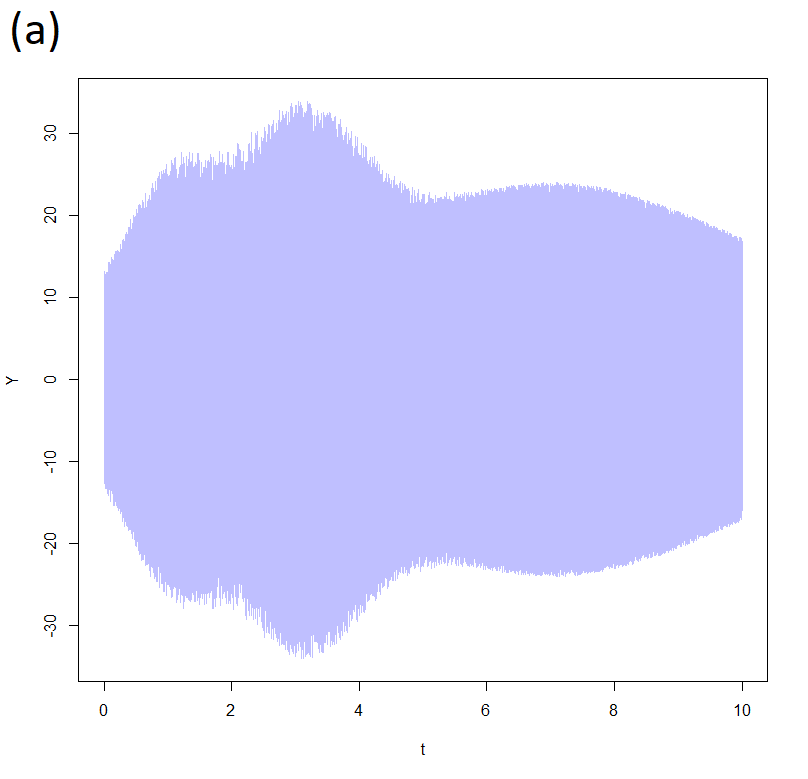
\includegraphics[width=\linewidth]{signal_build1.png}
 		\phantomsubcaption
 		\label{F1a}
 	\end{subfigure}
 	\hfill
 	\begin{subfigure}[t]{0.49\textwidth}
 		\centering
 		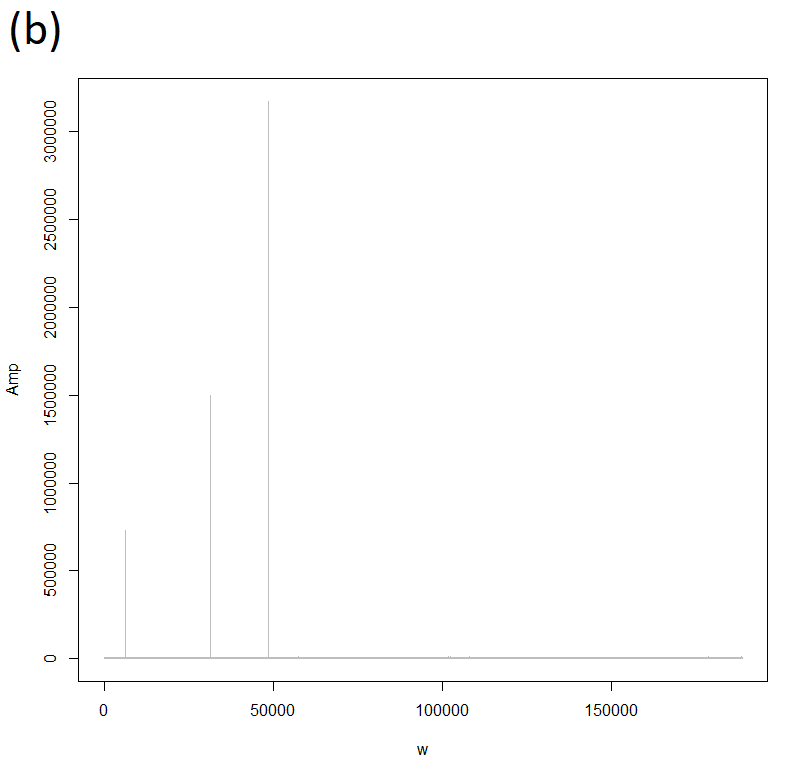
\includegraphics[width=\linewidth]{signal_build1_AmpSpec.png}
 		\phantomsubcaption
 		\label{F1b}
 	\end{subfigure}
 	\vfill
	\begin{subfigure}[t]{0.49\textwidth}
	\centering
	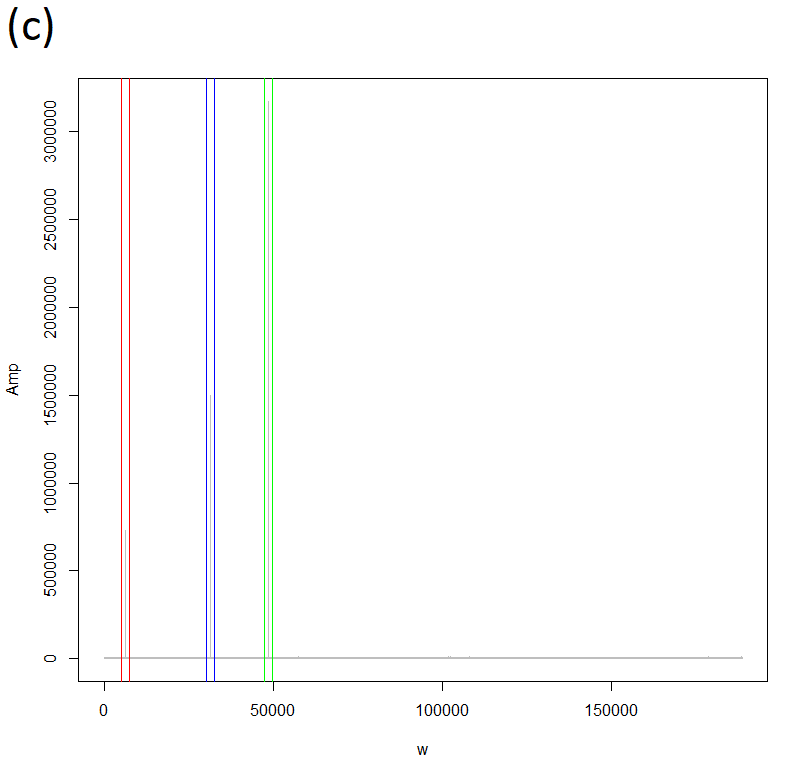
\includegraphics[width=\linewidth]{signal_build1_AmpSpec_Windows.png}
	\phantomsubcaption
	\label{F1c}
\end{subfigure}
\hfill
\begin{subfigure}[t]{0.49\textwidth}
	\centering
	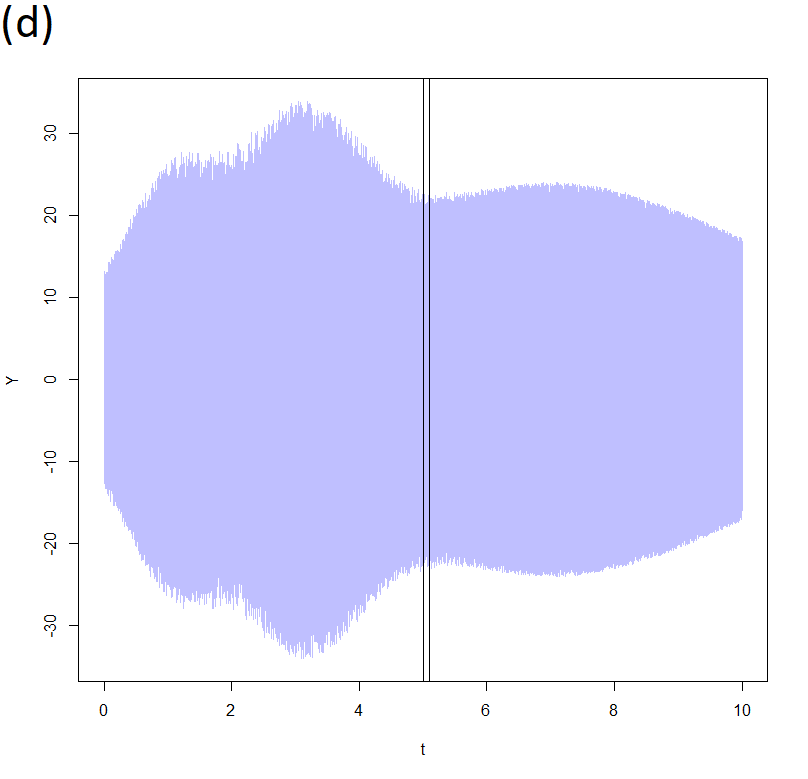
\includegraphics[width=\linewidth]{signal_build1_xbox_size.png}
	\phantomsubcaption
	\label{F1d}
\end{subfigure}
 	\caption{(a)Plot of $Y$ vs $t$ generated using R. (b)Amplitude spectra of the plot in (a). (c)frequency windows selected for the frequencies in (b). (d)real space xbox window size created for (a)}\label{F1}
 \end{figure}
As shown in fig.\ref{F1a}, a trimodal signal is visible and as is derived from the code in listing.\ref{lst:cb1} there exist only three frequencies in the  \lstinline[language=R]|fcomp| variable.
To check the mappings of the three frequency components in fig.\ref{F1b}, three frequency windows were created.
\pagebreak
 \begin{lstlisting}[language=R, label={lst:cb2}, caption={code for plotting the three frequency windows in fig.\ref{F1c}}, captionpos=b]
	##Plotting the frequency windows
	fY <- ft(t,Y,w=T) #function available with StatsChitran
	plot(fY$wf, abs(fY$fy), col= 'grey', typ='l', xlab='w', ylab='Amp')
	
	##for the 1000Hz freq
	abline(v=2*pi*800, col='red')
	abline(v=2*pi*1200, col='red')
	
	##for the 5000Hz freq
	abline(v=2*pi*4800, col='blue')
	abline(v=2*pi*5200, col='blue')
	
	##for the 7734Hz freq
	abline(v=2*pi*7534, col='green')
	abline(v=2*pi*7934, col='green')
\end{lstlisting}
As shown in listing.\ref{lst:cb2}, the code for plotting the lines around the relevant frequencies (see fig.\ref{F1c}) were used. The code for plotting the real-space window in fig.\ref{F1d} is shown in listing.\ref{lst:cb4}.\\
 As seen in listing.\ref{lst:cb2}, the frequency windows selected were $\omega = 2\pi(800 ---- 1200)$ for the 1000\si{Hz} peak, $\omega = 2\pi(4800 ---- 5200)$ for the 5000\si{Hz} peak and $\omega = 2\pi(7534 ---- 7934)$ for the 7734\si{Hz} peak rerspectively.\\
 Hence, the selected windows were equispaced in $f/\omega$ space with a $\Delta\omega = 2\pi \times 400$ fort each. This selection has consequences which will be shown.
 \subsubsection{Creating the data-structures required for the arguments of freq\_map()}
 $\bullet$ The \lstinline[language=R]|w_int| dataframe\\
 The function \textit{freq\_map()} first and foremost needs a \lstinline[language=R]|w_int| argument, which denotes the integration windows of the signals \textbf{in $\omega$-space}\footnote{Donot use $f$-space values in \lstinline[language=R]|w_int|, use ONLY $\omega$-space values, or else the results received will be incorrect}. \lstinline[language=R]|w_int| is always a $n$ column dataframe with two observations. Here $n$ is the no. of integrstion windows under consideration. For this case, as shown in listing.\ref{lst:cb2} and fig.\ref{F1c}, $n=3$, while the two observations are the two limits of the integration window shown in fig.\ref{F1c}
  \begin{lstlisting}[language=R, label={lst:cb3}, caption={code for the w\_int dataframe for the three frequency windows in fig.\ref{F1c}}, captionpos=b]
	##building the datasets for freq_map()
	#build dataframe for w_int (Integration window)
	w1 <- c(2*pi*800, 2*pi*1200)
	w2 <- c(2*pi*4800, 2*pi*5200)
	w3 <- c(2*pi*7534, 2*pi*7934)
	w_dat <- data.frame(w1, w2, w3)
 \end{lstlisting}
$\bullet$ The \lstinline[language=R]|xbox| number\\
The \textit{freq\_map()} function also needs to know the resolution of its window in real space as shown in fig.\ref{F1d}. \textbf{For this either \lstinline[language=R]|xbox| or \lstinline[language=R]|nbin| can be used}. The case with \lstinline[language=R]|xbox| is shown here.
\pagebreak
  \begin{lstlisting}[language=R, label={lst:cb4}, caption={code for the xbox number fig.\ref{F1d}}, captionpos=b]
	#build the xbox data(Box size in real space)
	box_len <- 0.1
	plot(t,Y, col=rgb(0,0,1,0.25), typ='l')
	abline(v=5, col='black')
	abline(v=5+box_len, col='black')
\end{lstlisting}
The argument \lstinline[language=R]|xbox| is simply a number in R as shown. The first \lstinline[language=R]|abline(v=5, col='black')| was chosen just for convenience of representation. What is important to know is that \lstinline[language=R]|box_len <- 0.1|. To show the comparative size of the window, the second vertical line was plotted using \lstinline[language=R]|abline(v=5+box_len, col='black')| (listing.\ref{lst:cb4}, fig.\ref{F1d})\\
\\
$\bullet$ The \lstinline[language=R]|color| vec\\
The \lstinline[language=R]|color| argument is a vector which is needed anytime a plot is required from \textit{freq\_map()}.
\lstinline[language=R]|color| is necessarily of length $n$ and a vector of colours\footnote{$n$ is the no. of integration windows or the no. of columns in \lstinline[language=R]|w_int|}. As shown in listing.\ref{lst:cb5}, the \lstinline[language=R]|color| argument is just a vector of colors.

\begin{lstlisting}[language=R, label={lst:cb5}, caption={vector of colours to use in the plot}, captionpos=b]
	#build the color vector(use only when plt=T)
	col_vec <- c('red','blue', 'green')
\end{lstlisting}
$\bullet$ Running the frequency mapping with \lstinline[language=R]|xbox|
\begin{lstlisting}[language=R, label={lst:cb6}, caption={Run the frequency map with xbox}, captionpos=b]
	##run the frequency mapping
	L <- freq_map(t,Y, w_int = w_dat, xbox = box_len, color = col_vec, plt = T, plt.leg = T)
\end{lstlisting}
\textit{freq\_map()} is run as shown in listing.\ref{lst:cb6}. The \lstinline[language=R]|plt.leg| command forces a legend on the graph when set to \lstinline[language=R]|TRUE|.\\
The  returned variable \lstinline[language=R]|L| is a list with length equal to $n$. Each index of the list contains the dataframes from the corresponding maps in \lstinline[language=R]|w_int|. The dataframe calculated as a result of the window \lstinline[language=R]|w_int[,i]| is present in \lstinline[language=R]|L[[i]]|.\\
  \\
$\bullet$ The \lstinline[language=R]|nbin| vector\\
The \textit{freq\_map()} can also be run with \lstinline[language=R]|nbin| \underline{instead of} \lstinline[language=R]|xbox|. The function throws an error when both arguments are provided simultaneously, because they are conflicting arguments.\\
The \lstinline[language=R]|nbin| argument denotes the no. of periodicities of each frequency window that will be used to calculate the resolution of the window in realspace.\footnote{There are consequences to using either \lstinline[language=R]|nbin| or \lstinline[language=R]|xbox|.} 
\begin{lstlisting}[language=R, label={lst:cb7}, caption={code for the nbin vector}, captionpos=b]
	#build the nbin vecor
	x_bin <- c(100,100,100)
\end{lstlisting}
As seen in lsiting.\ref{lst:cb7}, it is obvious that the length of \lstinline[language=R]|nbin| will be equal to $n$.\\
\pagebreak
  \\
$\bullet$ Running the frequency mapping with the \lstinline[language=R]|nbin| vector
\begin{lstlisting}[language=R, label={lst:cb8}, caption={Run the frequency map with nbin}, captionpos=b]
	##run the frequency mapping
	L <- freq_map(t,Y, w_int = w_dat, nbin = x_bin, color = col_vec, plt = T, plt.leg = T)
\end{lstlisting}
\subsubsection{Comparing the plots using xbox and nbin}
 \begin{figure}[h]
	\centering
	\begin{subfigure}[t]{0.49\textwidth}
		\centering
		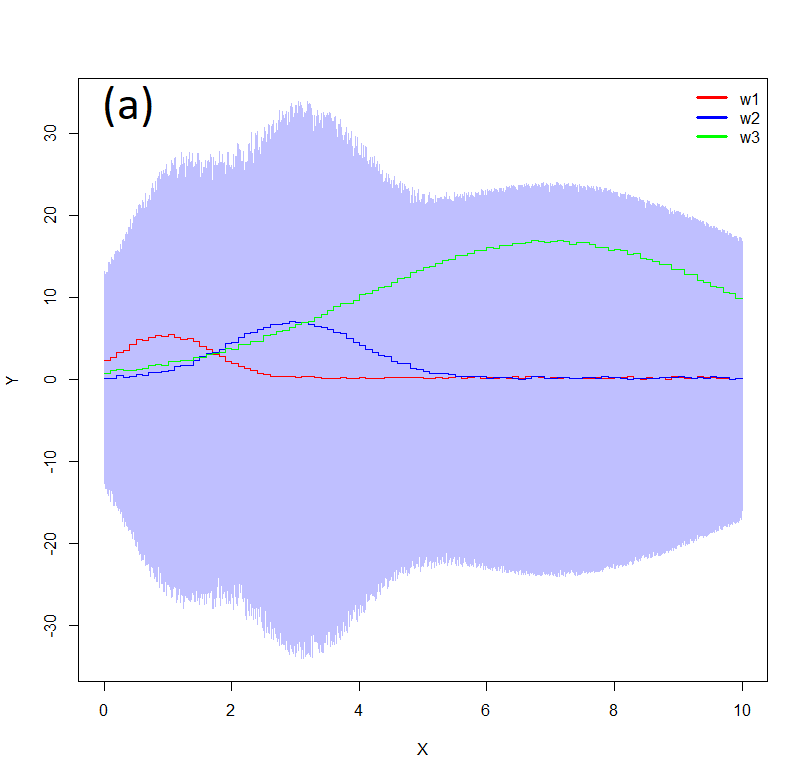
\includegraphics[width=\linewidth]{signal_build1_freqMap_xbox.png}
		\phantomsubcaption
		\label{F2a}
	\end{subfigure}
	\hfill
	\begin{subfigure}[t]{0.49\textwidth}
		\centering
		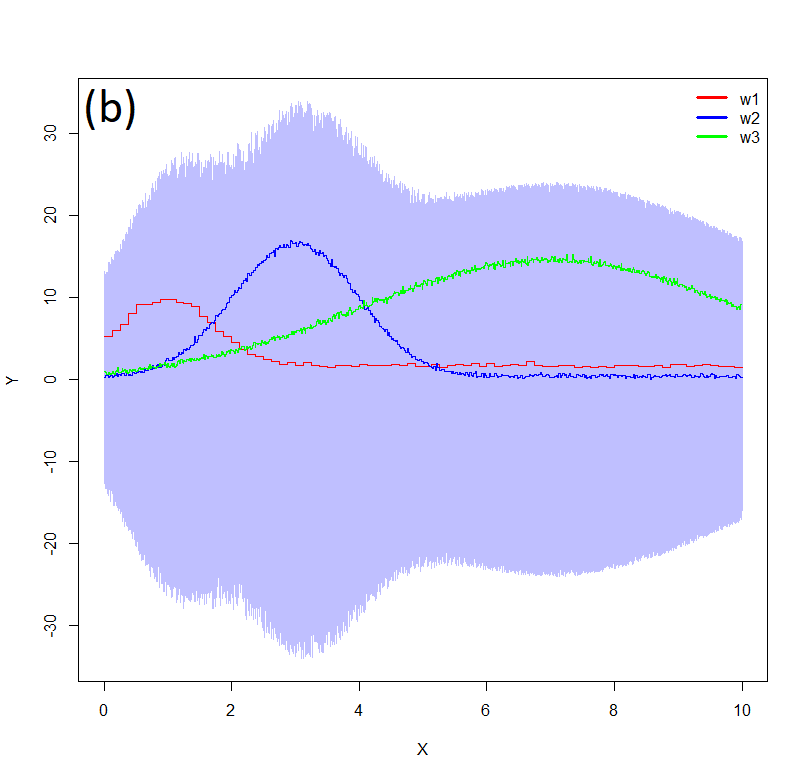
\includegraphics[width=\linewidth]{signal_build2_freqMap_nbin.png}
		\phantomsubcaption
		\label{F2b}
	\end{subfigure}
	\caption{Overlay \lstinline[language=R]|freq_map| plots showing contribution of individual frequency windows with (a)\lstinline[language=R]|xbox| and (b)\lstinline[language=R]|nbin| }\label{F2}
\end{figure}
As can be seen, the plots in fig.\ref{F2a} and fig.\ref{F2b} generated with \lstinline[language=R]|xbox| and \lstinline[language=R]|nbin| respectively. Both plots show the expected frequency distributions, but with slight difference. Using the \lstinline[language=R]|xbox| in fig.\ref{F2a}, we have equal resolution(bin sizes) on all three frequency windows $\omega_1, \omega_2$ and $\omega_3$, while with \lstinline[language=R]|nbin| in fig.\ref{F2b} we can see that the red curve ($\omega_1$) has a worse resolution than the blue curve, $\omega_2$, which in turn has a worse resolution than the green curve, $\omega_3$, but the overall shape provided by the distribution tend to fit the original trimodal distribution better.\\

Thus, \lstinline[language=R]|xbox| and \lstinline[language=R]|nbin| allow trade-offs.\\
$\bullet$ \lstinline[language=R]|xbox|:
\begin{itemize}
	\item Provides uniform real-space resolution for all frequency windows
	\item Intensity ratios of competing frequency windows distributions in real-space can't be trusted  
\end{itemize}
 \\
$\bullet$ \lstinline[language=R]|nbin|:
\begin{itemize}
	\item Intensity ratios of competing frequency windows distributions in real-space can be trusted
	\item Non-uniform resolution of real-space distributions from different frequency windows
\end{itemize}
This issue occurs, because different frequency windows have different wavelengths/Time periods and hence have a different number of waves/periods that can be fit into a given \lstinline[language=R]|xbox|, however with \lstinline[language=R]|nbin|, we can normalize for the number of waves/periods that we fit into our real space bins, but as a result have different bin sizes/resolution in real space.
\subsubsection{Proof of concept}
 
 \begin{figure}[h]
	\centering
	\begin{subfigure}[t]{0.32\textwidth}
		\centering
		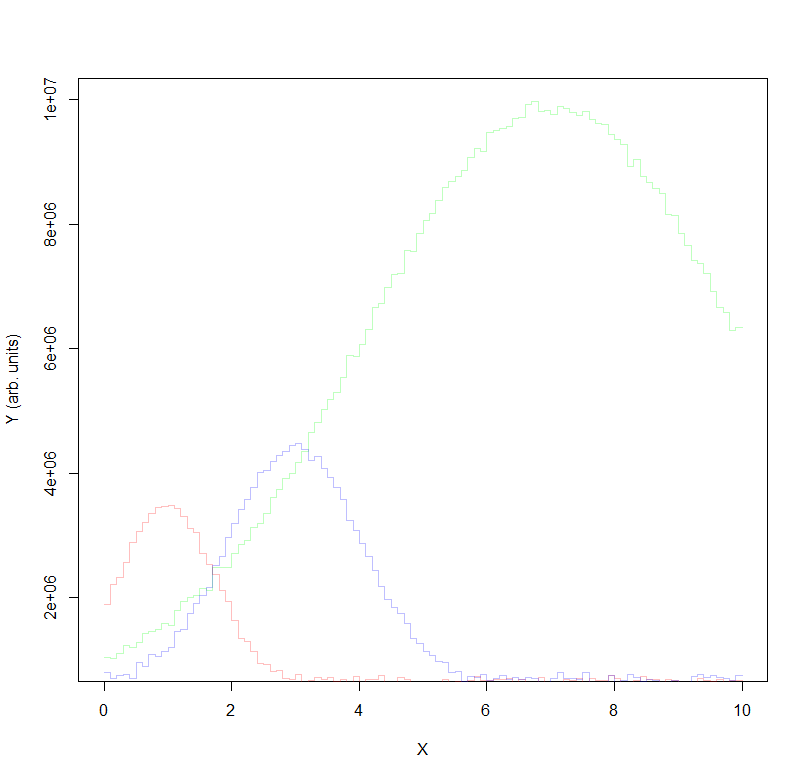
\includegraphics[width=\linewidth]{Proof_Concept_noisy_list_xbox.png}
		\phantomsubcaption
		\label{F3a}
	\end{subfigure}
	\hfill
	\begin{subfigure}[t]{0.32\textwidth}
		\centering
		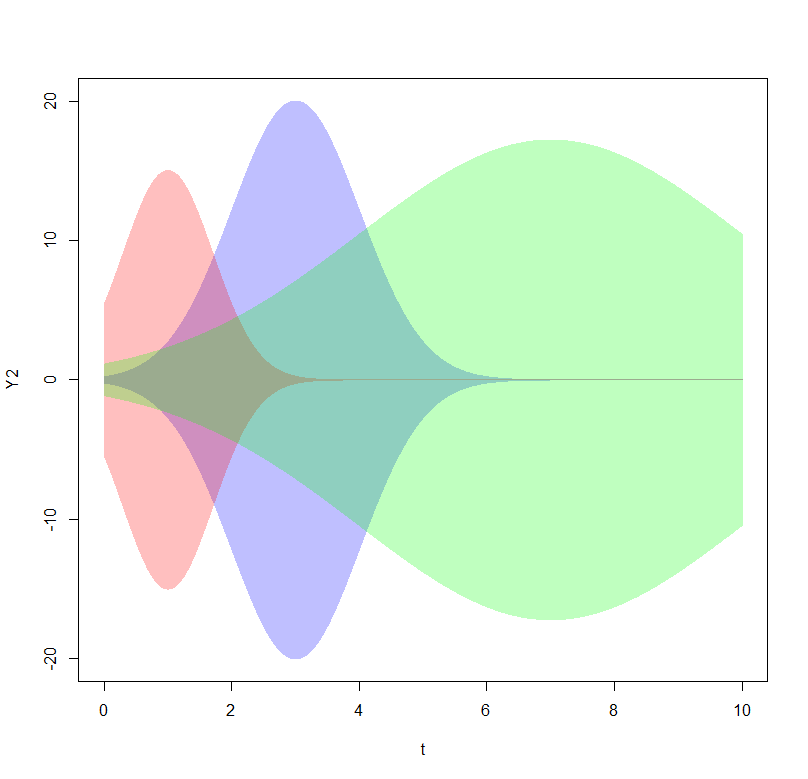
\includegraphics[width=\linewidth]{Proof_Concept_noiseless.png}
		\phantomsubcaption
		\label{F3b}
	\end{subfigure}
	\hfill
	\begin{subfigure}[t]{0.32\textwidth}
		\centering
		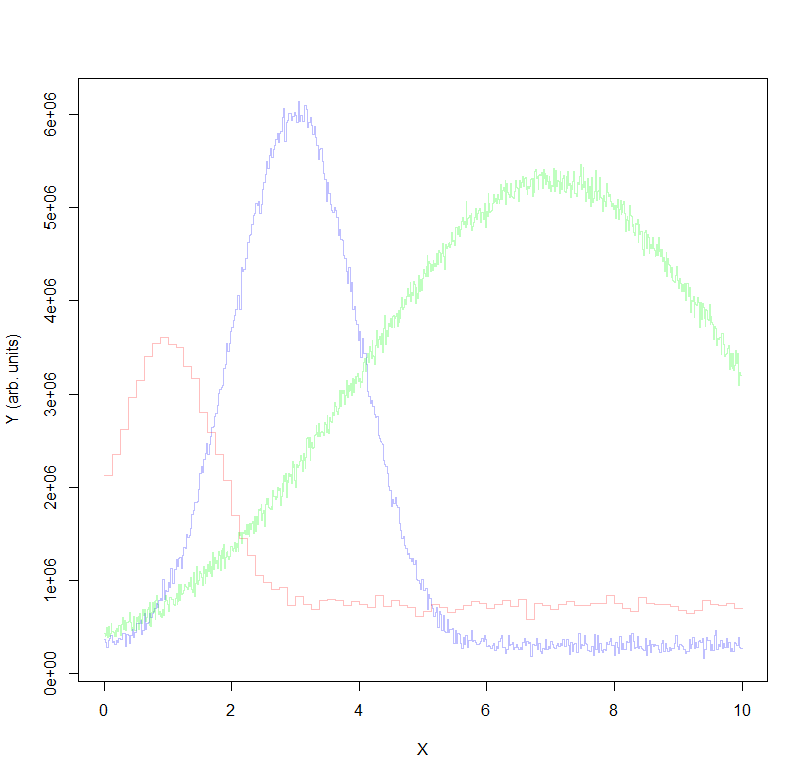
\includegraphics[width=\linewidth]{Proof_Concept_noisy_list_nbin.png}
		\phantomsubcaption
		\label{F3c}
	\end{subfigure}	
	\caption{(a)Plot of $t$ vs $Y$ data generated using \lstinline[language=R]|xbox| \ref{}. (b)Plot of $t$ vs $Y$ data generated using \ref{label}. (c)Plot of $t$ vs $Y$ data generated using \lstinline[language=R]|nbin| \ref{label}}\label{F3}
\end{figure}
\end{document}
